\chapter{Basic concepts}
Spot essentially manipulates $\omega$-automata which is a variation of finite-state automata (FSA) that runs
on infinite, rather than finite. It is important to have a good understanding of automata theory,
not only to understand this report but because automata crop up preety much everywhere in computer
science. In logic design, natural language processing, system analysis, regular expressions, etc. The next
two sections introduce the basics of automata theory and some concepts used in Spot.

\section{Automata theory}
\textit{Automata theory} \cite{9} is the study of abstract machines and automata, as well as the
computational problems that can be solved using them.

\begin{figure}[H]
 \centering
 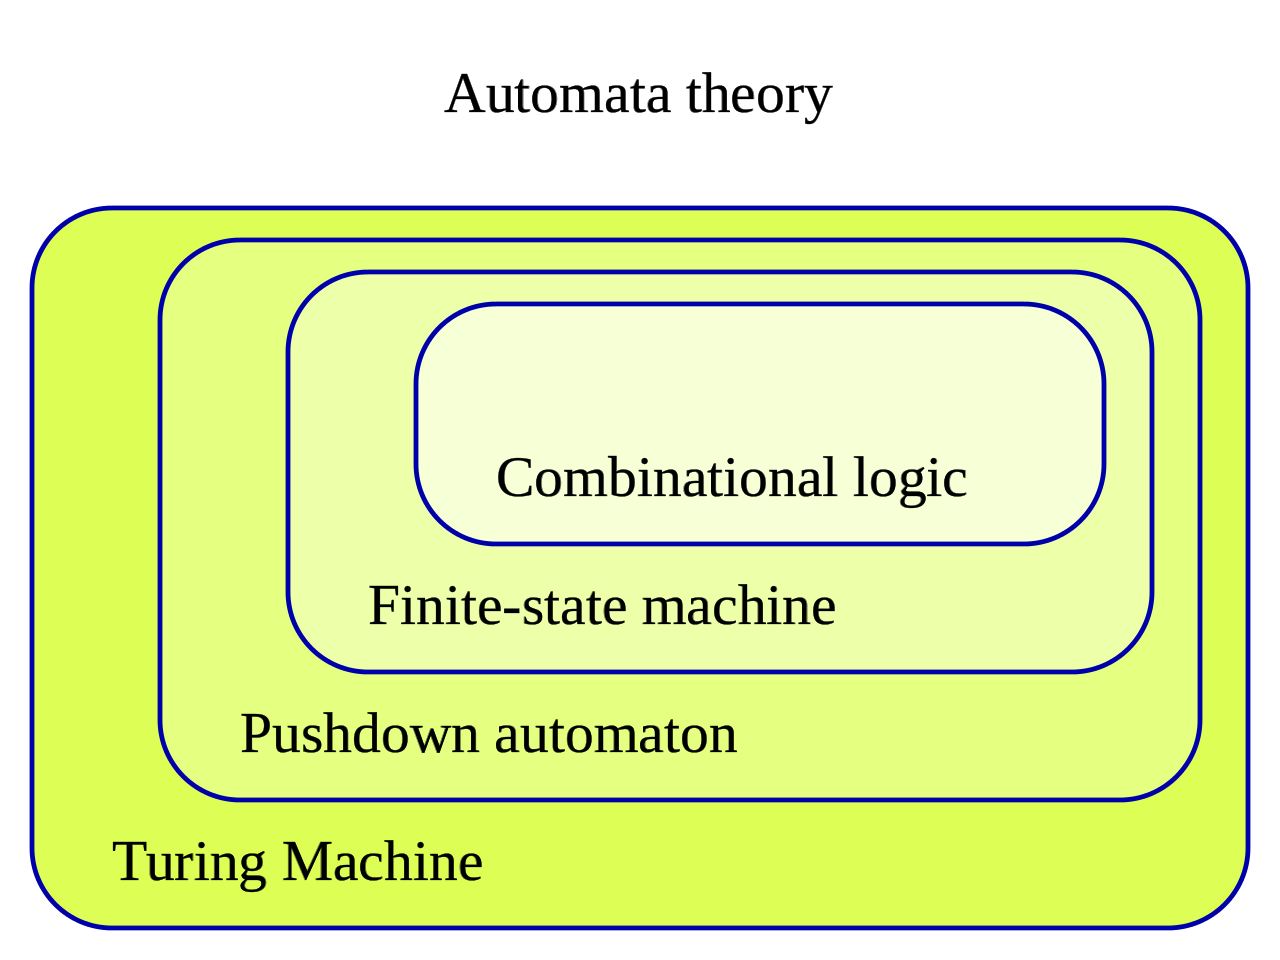
\includegraphics[scale=0.2]{img/automata_classes.png}
 \caption{Classes of automata \cite{9}}
 \label{fig:aut_classes}
\end{figure}
There are different classes of automata. The finite state machine has less computational power than
some other models of computation such as the Turing machine \cite{10}. The computational power distinction
means there are computational tasks that a Turing machine can do but a finite-state automaton (FSA) can
not.

\noindent From now on, the acronym FSA will be used instead of final-state automat\{a, on\}.

Only FSA will be concisely described in this section as (again) $\omega$-automata used in Spot are a
variation of FSA.

\subsection{Finite-state automata}
\begin{figure}[h]
  \centering
  \begin{tikzpicture}[shorten >=1pt,node distance=4cm,on grid,auto] 
    \node[state,initial] (q_0)   {$q_0$};
    \node[state, accepting] (q_1) [right=of q_0] {$q_1$};
    \path[->] 
    (q_0) edge[bend right=-30] node {$b$} (q_1)
          edge[loop above]     node {$a$} ()
    (q_1) edge[bend left=30]   node {$a$} (q_0)
          edge[loop above]     node {$b$} ();
  \end{tikzpicture}
  \caption{A finite-state automaton represented using a graph}
   \label{aut:pres}
\end{figure}

This figure (\ref{aut:pres}) shows how an automaton looks like. It consists of:
\begin{itemize}
 \item a set of states (represented in the figure by circles). Among them we can distinguish the 
       \textit{initial state} \textbf{q0} (the one pointed by \textbf{start}) and an
       \textit{accepting state} \textbf{q1} (the one doubly encircled).
 \item a transition relation (represented in the figure by arrows). This function indicates for each
       state which state could be next according to the next symbol to read.
\end{itemize}

Before giving a regular definition, some points need clarification.

\subsubsection{Alphabet, word, language}
An alphabet is a finite set of symbols. It is commonly denoted by $\Sigma$. Edges of automata are labeled
by those symbols. The alphabet used by the automaton of figure \ref{aut:pres} is $\{a, b\}$. \\

\noindent A word is a finite sequence of symbols. $a$, $b$, $ab$, $aaaa$, $abbba$, $ababababbbaaabbaba$ are
some words defined on the alphabet $\{a, b\}$. Automata recognizes words. In Spot, $\omega$-automata
recognizes \textit{$\omega$-words}, which are infinite rather than finite.\\

\noindent A language is a set of words defined on the same alphabet. The automata of figure \ref{aut:pres}
accepts or recognizes the set of words ending with $b$.

\subsubsection{Automaton run}
Well, an automaton run can be described as follows:
\begin{itemize}
 \item it starts in the initial state and waits for the first character (of the word) to read.
 \item At each step, it reads the next symbol (character) and determine the next state using the
       transition relation.
 \item It stops when all the character chain has been read. The word is accepted if the automaton is
       in one of the accepting states.
\end{itemize}

\subsubsection{Determinism}
A \textit{deterministic} FSA is a final state machine where for each pair of state and input (symbols)
there is one and only one transition to a next state. The figure \ref{aut:pres} introduced before is
actually a \textit{deterministic} FSA or \textit{deterministic} finite-state automaton (DFA).\\

\noindent A \textit{non deterministic} FSA allows:
\begin{itemize}
 \item many transitions labeled by the same symbol and outgoing from the same state,
 \item transitions labeled by the \textit{empty word} $\varepsilon$,
 \item transitions labeled by more than one symbol.
\end{itemize}


\subsubsection{Definition}
More formally, a finite-state automaton is defined by a quintuplet $M=(Q, \Sigma, X, s, F)$ where:
\begin{itemize}
 \item $Q$ is a set of states,
 \item $\Sigma$ is an alphabet,
 \item $X$ can be either a transition function $\delta : Q \times \Sigma \rightarrow Q$ (if the automaton is
       deterministic) or a transition relation $\Delta \subset (Q \times \Sigma^* \times Q)$ (if it is not
       deterministic),
 \item $s \in Q$ is the initial state,
 \item $F \subseteq Q$ is a set of accepting states.
\end{itemize}



\section{About Spot}
This section is a resume of Spot \textbf{concept} web page \cite{8}.

\subsection{Atomic preposition}
An \textit{atomic proposition} is a named Boolean variable that represents a simple property that must be
true or false. It usually represents some property of a system.

\subsection{Boolean formula}
A Boolean formula is formed from \textit{atomic preposition}, the Boolean constants true and false, and
standard Boolean operators like and, or, implies, xor, etc.